
\newgeometry{total={210mm,297mm},left=20mm,right=20mm,bindingoffset=5mm, top=25mm,bottom=25mm} 
\begin{partwithabstract}{\hspace{2mm}Results \& Experiments\label{part:results}}
    \par{
    The objective of this modelling procedure is to procedure a model that can estimate segmentation masks for the 5 lumbar vertebrae from \acrfull{ct} and \acrfull{mri} scans of human patients, 
    based on point annotation of these 6 classes ($L1$ to $L5$ and 1 background class).
}
\par{
    First, as described in chapter \ref{sec:reference_model}, a reference is calculated with which to compare the performance of the weakly supervised models.
    The reference models have the same architecture and are trained with full annotation on the same dataset as the weakly supervised models. 
}
\par{
    The first step in the modelling procedure based on point annotation masks is the construction of \textit{single-dimension} models.
    Single-dimension indicates that these models investigate the performance of a model that outputs 2D segmentation masks based on 2D input images.
    By slicing the scan volumes along one of three central dimensional axes, a stack of two-dimensional images is created together with the point annotation maps extracted from the segmentation masks of these images.
    Chapter \ref{sec:singleDimension} presents the results of several experiments. 
    Different model hyperparameters are tested.
    Models with different loss functions are trained on point annotation maps where the number of annotation points extracted from the full masks is varied.
}
\par{
    the second step in the modelling procedure is the combination of the single-dimension models to estimate pseudo-masks.
    These pseudo masks can finally be used to train a model as pseudo full annotation masks.
    Chapter \ref{sec:combination} first discusses the technique used to combine single-dimension models and then concludes with the results obtained by training a final model on the pseudo masks resulting from the combination.
}
\end{partwithabstract}
\restoregeometry

\chapter{Datasets}

This thesis is based on 5 different already existing datasets.
This chapter discusses these datasets based on different criteria:

\begin{description}
    \item[source:] reference of the owner of the dataset and brief description of the original purpose of the dataset. Importantly, this part also discusses the source of the annotation.
    \item[Patient sample:] statistics of the patients of whom medical images were collected such as age, gender and possible spine pathologies.
    \item[Technical information:] discusses the imaging technology, the image resolution and the spatial dimensions of the image. 
\end{description}

\section{Global overview of the different dataset}

\todo[inline]{Overview of the datasets gathered. MRI / CT, number of images, type of annotation + WHO performed the annotation? Was it a medical docter or one of the researchers.}



bla

\begin{SCtable}[\sidecaptionrelwidth][h]
 
    \begin{tabular}{ l l l l l} 
     \hline
     \hline
     Name & reference & imaging & Quantity & Annotation \\
          &           & technology & [images] & \\
     \hline 
    UWSpine & \cite{Glocker}  & \acrshort{ct} & 125 & point  \\ 
    xVertSeg & \cite{Ibragimov2014, Korez2015} & \acrshort{ct} & 15 & full \\
    UniSiegen  & \cite{Zukic2014} & \acrshort{mri} & 17 & full \\
    PLoS & \cite{Chu2015} & \acrshort{mri} & 23 & semantic \\
    MyoSegmenTUM & \cite{Burian2019} & \acrshort{mri} &  54 & full \\
     \hline
     \hline
    \end{tabular}
    \caption{List of dataset references. For more details on the data quantity, please consult chapter \ref{seg:datasetcomparison}. 
    Notably the fact that some images were taken from the same patient is important. This means the dataset is grouped. 
    The agreement with prof. T. Vrtovec regarding the xVertSeg dataset can be found in appendix \ref{seg:datasetagreement}.}

\end{SCtable}

\begin{SCtable}[\sidecaptionrelwidth][h]
 
    \begin{tabular}{ l l l l} 
     \hline
     \hline
     Name & X & Y & Z \\
     \hline 
    UWSpine & Left-right & Anteroposterior & Craniocaudal \\
    xVertSeg & Left-right & Anteroposterior & Craniocaudal \\
    UniSiegen  &  Anteroposterior & Craniocaudal & Left-right \\
    PLoS & Left-right & Anteroposterior & Craniocaudal$^\dagger$ \\
    MyoSegmenTUM &  Anteroposterior & Craniocaudal & Left-right \\
     \hline
     \hline
    \end{tabular}
    \caption{List of dataset references. For more details on the data quantity, please consult chapter \ref{seg:datasetcomparison}. 
    Notably the fact that some images were taken from the same patient is important. This means the dataset is grouped. 
    The agreement with prof. T. Vrtovec regarding the xVertSeg dataset can be found in appendix \ref{seg:datasetagreement}.
    $^\dagger$ The Craniocaudal axis in the PLoS dataset is inverted.}

\end{SCtable}

\section{Comparison of the different datasets\label{seg:datasetcomparison}}


\subsection{xVertSeg\label{sec:xVertSeg}}



The xVertSeg \cite{Ibragimov2012, xxx} was kindly made available by prof. T. Vrtovec (University of Ljubljana, Faculty of Electrical Engineering, Slovenia), see appendix \ref{seg:datasetagreement} for the agreement.
This dataset contains 25 \acrfull{ct} scans of the lumbar spine, of which 15 \acrshort{ct} scans are fully labeled.
Given the provided data, I can assume these 15 scans were collected from 15 different patients.

For each of these 15 scans, full instance segmenation masks for all 5 lumbar vertebrae are provided. The delineation was performed by a skilled professional.

Additionally, for each vertebra a fracture class and fracture grade is provided. 
Apart from vertebrae classified as \textit{normal}, the dataset contains \textit{mild}, \textit{moderate} and \textit{severe} cases of vertebrae fracture types \textit{wedge}, \textit{crush} and \textit{biconcavity}.
\marginpar{
        % This file was created by tikzplotlib v0.9.8.
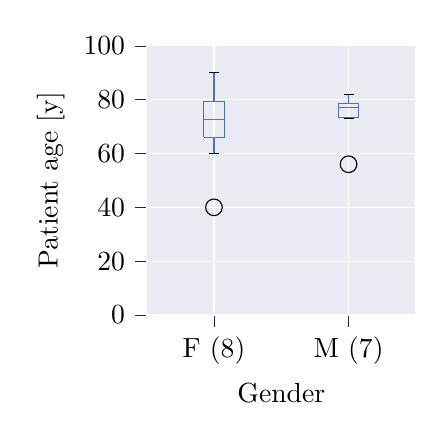
\begin{tikzpicture}

\definecolor{color0}{rgb}{0.917647058823529,0.917647058823529,0.949019607843137}
\definecolor{color1}{rgb}{0.298039215686275,0.447058823529412,0.690196078431373}
\definecolor{color2}{rgb}{0.768627450980392,0.305882352941176,0.32156862745098}

\begin{axis}[
axis background/.style={fill=color0},
axis line style={white},
height=5cm,
tick align=outside,
tick pos=left,
width=5cm,
x grid style={white},
xlabel={Gender},
xmajorgrids,
xmin=0.5, xmax=2.5,
xtick style={color=white!15!black},
xtick={1,2},
xticklabels={F (8),M (7)},
y grid style={white},
ylabel={Patient age [y]},
ymajorgrids,
ymin=0, ymax=100,
ytick style={color=white!15!black}
]
\addplot [color1, opacity=1]
table {%
0.925 66
1.075 66
1.075 79.25
0.925 79.25
0.925 66
};
\addplot [color1, opacity=1]
table {%
1 66
1 60
};
\addplot [color1, opacity=1]
table {%
1 79.25
1 90
};
\addplot [black, opacity=1]
table {%
0.9625 60
1.0375 60
};
\addplot [black, opacity=1]
table {%
0.9625 90
1.0375 90
};
\addplot [black, mark=o, mark size=3, mark options={solid,fill opacity=0}, only marks]
table {%
1 40
};
\addplot [color1, opacity=1]
table {%
1.925 73.5
2.075 73.5
2.075 78.5
1.925 78.5
1.925 73.5
};
\addplot [color1, opacity=1]
table {%
2 73.5
2 73
};
\addplot [color1, opacity=1]
table {%
2 78.5
2 82
};
\addplot [black, opacity=1]
table {%
1.9625 73
2.0375 73
};
\addplot [black, opacity=1]
table {%
1.9625 82
2.0375 82
};
\addplot [black, mark=o, mark size=3, mark options={solid,fill opacity=0}, only marks]
table {%
2 56
};
\addplot [color2, opacity=1]
table {%
0.925 72.5
1.075 72.5
};
\addplot [color2, opacity=1]
table {%
1.925 77
2.075 77
};
\end{axis}

\end{tikzpicture}

        \captionof{figure}{xVertSeg patients age distribution}
        \label{fig:xVertSeg_Age}
    }

\subsubsection{Original Objective of the Dataset}

The objective of the \textit{xVertSeg challenge}\footnote{see \url{http://lit.fe.uni-lj.si/xVertSeg/database.php}} (2015) was organized by the University of Ljubljana.
Based on the 15 provided scans with corresponding masks, the participans were required to construct a model to make predictions on the test set of 10 unlabelled scans.

The challenge consisted of two tasks:
\begin{enumerate}
    \item Segmentation of the lumbar vertebrae. For each scan in the test set, the segmentation masks of the lumbar vertebrae were requested.
    \item Fracture classification on the segmented vertebrae, consisting of morphological grade and fracture classification.
\end{enumerate}

\subsubsection{Patient statistics}

The patients in the xVertSeg dataset train set consist of 8 females and 7 males.
The age of these patients is slightly higher than for the other datasets.
The average patient in this dataset is 71 years old.
A box plot of the age distribution between genders is shown in figure \ref{fig:xVertSeg_Age}. 

\begin{SCtable}[\sidecaptionrelwidth][h]
    \centering
        \begin{tabular}{lrrrrrr}
\toprule
{} &  L1 &  L2 &  L3 &  L4 &  L5 &  Total \\
\midrule
biconcave &   6 &   7 &   8 &   4 &   2 &     27 \\
normal    &   5 &   6 &   4 &   4 &   7 &     26 \\
wedge     &   3 &   2 &   2 &   3 &   2 &     12 \\
crush     &   1 &   0 &   1 &   4 &   4 &     10 \\
\bottomrule
\end{tabular}

        \caption{Every patient in the xVertSeg dataset suffers from at least one spine pathology.
        Most of these pathologies are identified as \textit{mild}.
        This table counts the spine pathologies and normal vertebrae observed over all 15 patients in the xVertSeg dataset.}   
\end{SCtable}

\subsubsection{Technical information}

The xVertSeg dataset contains 15 \acrshort{ct} annotated scans. 
This dataset is very interesting due to the high quality and high resolution of the images.
On figure \ref{fig:xVertSeg_image002}, two slices of the same patient (002) are represented.
The slices show the complete, uncropped sections of the torso and abdominal region of the patient. 
There is no \acrshort{roi} cropping.

\begin{SCfigure}[][htb]
    \centering
    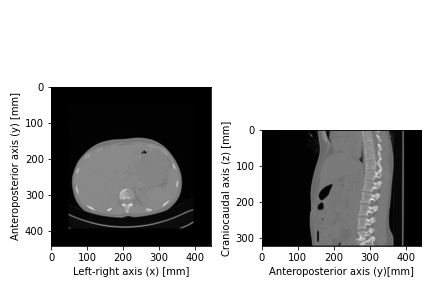
\includegraphics[width=.95\textwidth]{automated_graphs/xVertSeg_image002.png}
    \caption{xVertSeg scan \textit{image002}. \label{fig:xVertSeg_image002}}
\end{SCfigure}

The distribution of the scan dimensions is shown in figure \ref{fig:AllDataset_dims}. This also illustrates the \textit{xVertSeg} dataset consists of large, high resolution images.
Mind that during pre-processing the scans are resampled on a $1mm \times 1mm \times 1mm$ grid.


\subsection{UniSiegen dataset\label{sec:DataUSiegen}}

This dataset is made available in 2014 by the University of Siegen, Germany.
Dr D. Zukic \cite{Zukic2014} constructed it as part of his PhD project.

\marginpar{
        % This file was created by tikzplotlib v0.9.8.
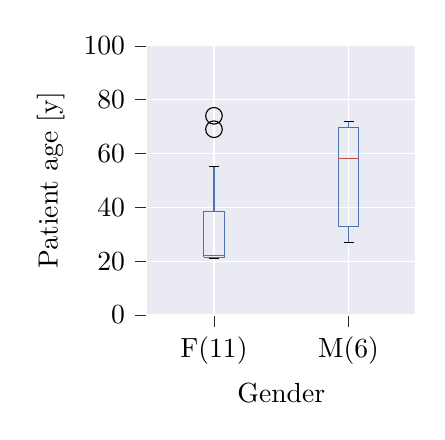
\begin{tikzpicture}

\definecolor{color0}{rgb}{0.917647058823529,0.917647058823529,0.949019607843137}
\definecolor{color1}{rgb}{0.298039215686275,0.447058823529412,0.690196078431373}
\definecolor{color2}{rgb}{0.768627450980392,0.305882352941176,0.32156862745098}

\begin{axis}[
axis background/.style={fill=color0},
axis line style={white},
height=5cm,
tick align=outside,
tick pos=left,
width=5cm,
x grid style={white},
xlabel={Gender},
xmajorgrids,
xmin=0.5, xmax=2.5,
xtick style={color=white!15!black},
xtick={1,2},
xticklabels={F(11),M(6)},
y grid style={white},
ylabel={Patient age [y]},
ymajorgrids,
ymin=0, ymax=100,
ytick style={color=white!15!black}
]
\addplot [color1, opacity=1]
table {%
0.925 21.5
1.075 21.5
1.075 38.5
0.925 38.5
0.925 21.5
};
\addplot [color1, opacity=1]
table {%
1 21.5
1 21
};
\addplot [color1, opacity=1]
table {%
1 38.5
1 55
};
\addplot [black, opacity=1]
table {%
0.9625 21
1.0375 21
};
\addplot [black, opacity=1]
table {%
0.9625 55
1.0375 55
};
\addplot [black, mark=o, mark size=3, mark options={solid,fill opacity=0}, only marks]
table {%
1 74
1 69
};
\addplot [color1, opacity=1]
table {%
1.925 33
2.075 33
2.075 69.5
1.925 69.5
1.925 33
};
\addplot [color1, opacity=1]
table {%
2 33
2 27
};
\addplot [color1, opacity=1]
table {%
2 69.5
2 72
};
\addplot [black, opacity=1]
table {%
1.9625 27
2.0375 27
};
\addplot [black, opacity=1]
table {%
1.9625 72
2.0375 72
};
\addplot [color2, opacity=1]
table {%
0.925 22
1.075 22
};
\addplot [color2, opacity=1]
table {%
1.925 58
2.075 58
};
\end{axis}

\end{tikzpicture}

        \captionof{figure}{USiegen patients age distribution}
        \label{fig:USiegen_Age}
    }

This dataset contains 26 \acrshort{mri} scans of 17 different patients\footnote{This is not clearly stated, but can be inferred from the metadata.}. 
The fact that scans of the same patient are correlated will be taken into account in the train, validation and test split.
For more details on this split, see section \ref{sec:trainValTestSplit} on page \pageref{sec:trainValTestSplit}.

\subsubsection{Original Objective of the Dataset}

This dataset was collected from several hospitals (Sarajevo, Marburg, Brisbane, Schwabach, Bad Wildungen \& Prague). The MRI scanner settings were varied between the scans (T1, T2, TIRM).
The PhD project objective was to build a segmentation model to automate the segmentation of the lumbar vertebrae in the \acrshort{mri} scans to facilitate the diagnosis of several spine pathologies 
such as scoliosis, spondylolisthesis \footnote{Spondylolisthesis is the displacement of one spinal vertebra compared to another.} and vertebral fractures.
The final model developed by dr. D. Zukic consisted of a Viola-Jones detector for detection and vertebral body size approximation.
The average Dice score compared to the manual reference was reported to be 79.3\%.

\subsubsection{Patient statistics}

In \cite{Zukic2014}, it is not entirely made clear which scans are taken from the same patient.
It is made clear, however that the 26 scans were not obtained from 26 patients.
The information was inferred from the naming of the scans and the provided gender en age information\footnote{
    Wrongfully assuming two scans come from the same patient does not cause data leakage.
}.

Figure \ref{fig:USiegen_Age} illustrates that the USiegen dataset contains almost double the number of female patients compared to male patients.
These patients are relatively young compared to the patients in the \textit{xVertSeg} dataset.

Only three of the patients in this dataset were categorized as having no spinal pathologies.

\subsubsection{Technical information}

Several \acrlong{mri} techniques were used to obtain the dataset: T1, T2 \& TIRM.
I do not take into account this factor in the model development or the dataset split.

The volumes in the USiegen dataset are strongly cropped. 
Both in the anteroposterior and the craniocaudal direction, the volumes are on average 370 mm.
In the left-right direction, however, the volumes have been cropped severely. The volumes are, on average, only 68 mm wide.
The images have been cropped to only include the \acrshort{roi}.
Along this left-right dimension, the voxel spacing is large. 

\begin{SCfigure}[][htb]
    \centering
    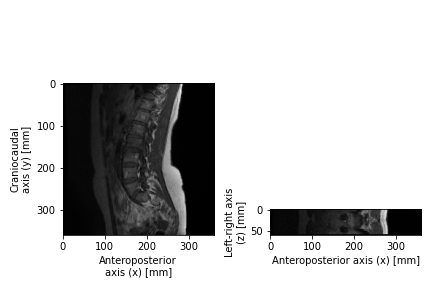
\includegraphics[width=.95\textwidth]{automated_graphs/USiegen_Aka3.png}
    \caption{USiegen dataset scan \textit{Aka3}. \label{fig:USiegen_Aka3}. It is immediately clear the USiegen volumes are cropped differently than the xVertSeg volumes.
    In the craniocaudal direction, both sacrum and coccyx are visible. Along the left-righ axis, the volumes have been cropped severely.}
\end{SCfigure}

The original scans in the \textit{USiegen} dataset were cropped in the \textit{left-right} direction. 
Although the scan resolution is relatively high in the Sagittal planes, the slice spacing along the left-right axis is coarser (see figure \ref{fig:AllDataset_dims}).  
\subsection{PLoS Dataset}

The \textit{PLoS} dataset was compiled for \cite{Chu2015} in 2015 by dr. C. Chu, University of Bern, Bern, Switzerland and made publically available \footnote{See : \url{ http://doi.org/10.5281/zenodo.22304 }} .
It consists of 23 T2-weighted spine \acrshort{mri} scans. 
Contrary to other datasets, the segmenation labels in this dataset do not provide information to destinguish the individual vertebrae from each other.

\subsubsection{Original Objective of the Dataset}

In \cite{Chu2015} the development of a random forest regression approach for spine vertebrae segmenation and classificiation is described.
The results of several random forest regressors and classifiers is unified with a voting mechanism.
This approach obtains a mean Dice metric score of 88.7\%.

\subsubsection{Patient statistics}

Due to the anomimization process, the \textit{PLoS} dataset does not contain patient information.
This means that it is not possible to produce any statistics regarding patient age or gender.

\subsubsection{Technical information}

As is indicated in figure \ref{fig:AllDataset_dims}, and in figure \ref{fig:PLoS_img02}, the PLoS image volumes are cropped in the left-right direction.
The volumes are consistently $381mm \times 381 mm \times 78 mm$, where the shortest dimension is in the left-right direction.

\begin{SCfigure}[][htb]
    \centering
    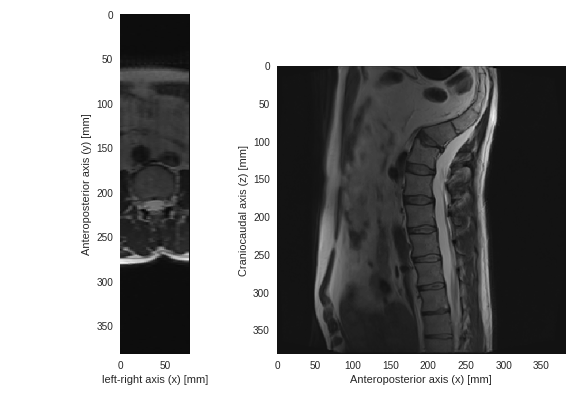
\includegraphics[width=.95\textwidth]{automated_graphs/PLoS_img02.png}
    \caption{
        PLoS dataset scan \textit{img02}. \label{fig:PLoS_img02}. The craniocaudal direction is cropped in a way comparable to the volumes in the USiegen dataset, but, the direction of this axis is inverted.
        The left-right axis is cropped similar to the USiegen data volumes.
    }
\end{SCfigure}
\subsection{MyoSegmenTUM datset}

This dataset is made available by S. Schläger from the Technische Universität München via the \acrfull{osf} \footnote{see \url{ https://osf.io/3j54b/?view_only=f5089274d4a449cda2fef1d2df0ecc56 }}.
It was constructed for the MyoSegmenTUM project \cite{Burian2019}.
It consists of 54 collections of \acrshort{mri} scans of the spine.
In this work, only the T2 weighted \acrlong{mri} scans are used.
The dataset also contains volumes with enhanced fat tissue response. Since the objective of this work is related to bone tissue rather than fat tissue, these volumes were not used.
Neither was the segmentation masks for the different dorsal muscles, which are also present in this dataset.

\subsubsection{Original Objective of the Dataset}

The MyoSegmenTUM Spine dataset is compiled as a reference dataset for developing segmentation algorithms of the lumbar spine vertebral bodies and muscle groups.
Information about this project can be found in \cite{Burian2019}.

\subsubsection{Patient statistics}

In figure \ref{fig:OSF_ageboxplot}, the age distribution of the patients in the MyoSegmenTUM dataset is shown.
There are more women (39) included in this dataset than men (15).
The male patients in this dataset are, on average, clearly younger than the female patients.

\marginpar{
        % This file was created by tikzplotlib v0.9.8.
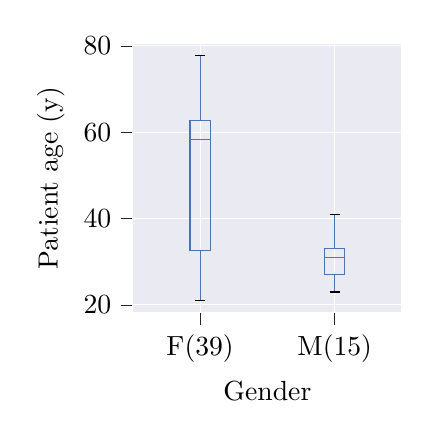
\begin{tikzpicture}

\definecolor{color0}{rgb}{0.917647058823529,0.917647058823529,0.949019607843137}
\definecolor{color1}{rgb}{0.298039215686275,0.447058823529412,0.690196078431373}
\definecolor{color2}{rgb}{0.768627450980392,0.305882352941176,0.32156862745098}

\begin{axis}[
axis background/.style={fill=color0},
axis line style={white},
height=5cm,
tick align=outside,
tick pos=left,
width=5cm,
x grid style={white},
xlabel={Gender},
xmajorgrids,
xmin=0.5, xmax=2.5,
xtick style={color=white!15!black},
xtick={1,2},
xticklabels={F(39),M(15)},
y grid style={white},
ylabel={Patient age (y)},
ymajorgrids,
ymin=18.1666324435318, ymax=80.5007186858316,
ytick style={color=white!15!black}
]
\addplot [color1, opacity=1]
table {%
0.925 32.5
1.075 32.5
1.075 62.7652292950034
0.925 62.7652292950034
0.925 32.5
};
\addplot [color1, opacity=1]
table {%
1 32.5
1 21
};
\addplot [color1, opacity=1]
table {%
1 62.7652292950034
1 77.6673511293635
};
\addplot [black, opacity=1]
table {%
0.9625 21
1.0375 21
};
\addplot [black, opacity=1]
table {%
0.9625 77.6673511293635
1.0375 77.6673511293635
};
\addplot [color1, opacity=1]
table {%
1.925 27
2.075 27
2.075 33
1.925 33
1.925 27
};
\addplot [color1, opacity=1]
table {%
2 27
2 23
};
\addplot [color1, opacity=1]
table {%
2 33
2 41
};
\addplot [black, opacity=1]
table {%
1.9625 23
2.0375 23
};
\addplot [black, opacity=1]
table {%
1.9625 41
2.0375 41
};
\addplot [color2, opacity=1]
table {%
0.925 58.2888432580424
1.075 58.2888432580424
};
\addplot [color2, opacity=1]
table {%
1.925 31
2.075 31
};
\end{axis}

\end{tikzpicture}

        \captionof{figure}{Distribution of patient age in the dataset from the MyoSegmenTUM project.}
        \label{fig:OSF_ageboxplot}
    }


\subsubsection{Technical information}

As shown in figure \ref{fig:OSF_02}, coupes from the second volume of the MyoSegmenTUM dataset are shown.
As is also indicated in figure \ref{fig:AllDataset_dims}, the dimensions of the MyoSegmenTUM volumes is consistent $220 mm \times 220 mm \times 80 mm$, where the shortest dimension is the cropped left-right axis.
There are only three volumes that deviate slightly from this.

\begin{SCfigure}[][htb]
    \centering
    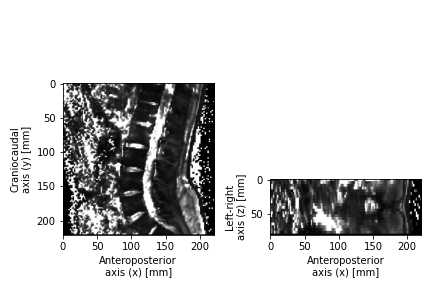
\includegraphics[width=.95\textwidth]{automated_graphs/OSF_02.png}
    \caption{MyoSegmenTUM dataset scan \textit{02}. 
    The volumes are cropped in the left-right direction. 
    \label{fig:OSF_02}}
\end{SCfigure}

\textbf{Remark:} For three volumes (nr 33, 53 and 54) for which the dimension of the image volume and the label mask do not correspond. 
It is not clear how these masks should be used. 
These volumes were discarded, bringing the final number of volumes used from the MyoSegmenTUM dataset to 51.
\subsection{UWSpine dataset}
 
This dataset is made available by the Department of Radiology of the University of Washington\footnote{Creative Commons Attribution-NonCommercial-NoDerivatives 4.0 International License, dataset available at \url{
      https://biomedia.doc.ic.ac.uk/data/spine/  
    }}.
It has been constructed by dr. Glocker and team \cite{Glocker2012,Glocker2013} (Microsoft research) in 2012.
For each scan, manual annotations of vertebrae centroids are provided.
This dataset contains 242 \acrshort{ct} scans of 150 different patients.
This dataset does not contain full mask labels, only centroid point annotations.
To investigate the relative performance of a weakly supervised model compared to the performance of a fully supervised model, both will be trained on the same dataset\footnote{The modelling concept is further discussed in chapter \ref{sec:model_concept}.}.
Furthermore, the evaluation of the models is based on the full annotations.
Thus, the UWSpine dataset will not be used for model training.
It will only be used for visual evaluation of the model on a completely new dataset\footnote{The UWSpine dataset is \textit{completely} new in the sense that no samples from this dataset (this \textit{population}, so to speak) are present in the train or validation set.
For the \textit{normal} test set, other samples from the same datasets where present in the train and validation sets.}.


\subsubsection{Original Objective of the Dataset}

In \cite{Glocker2012,Glocker2013} the development of a model based on regression forests and a \acrfull{hmm} for vertebra localisation without needing strong assumptions on what part of the spine is visible.

\subsubsection{Patient statistics}


Figure \ref{fig:UW_ageboxplot} illustrated that the patients in the \textit{UWSpine} dataset are relatively varied in age.
Of most patients in the dataset, multiple scan images are available.
The highest number of scans taken from a single patient is 5.

\subsubsection{Technical information}

Only point annotations are available for the \textit{UWSpine} dataset. 
This means this dataset can only be used for weakly supervised model training.

The scans in the \textit{UWSpine} dataset are strongly cropped around the spine, both in the left-right direction and the anteroposterior direction.

\begin{SCfigure}[][htb]
    \centering
    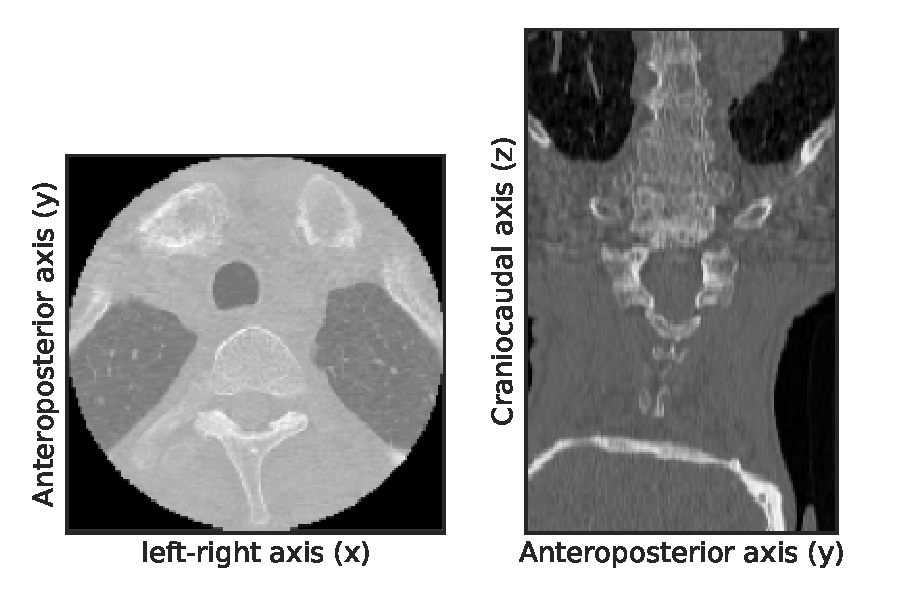
\includegraphics[width=.95\textwidth]{automated_graphs/UW_4564688.pdf}
    \caption{University of Washington dataset, scan \textit{4564688}. \label{fig:UW_4564688}}
\end{SCfigure}

\marginpar{
        % This file was created by tikzplotlib v0.9.8.
\begin{tikzpicture}

\definecolor{color0}{rgb}{0.917647058823529,0.917647058823529,0.949019607843137}
\definecolor{color1}{rgb}{0.298039215686275,0.447058823529412,0.690196078431373}
\definecolor{color2}{rgb}{0.768627450980392,0.305882352941176,0.32156862745098}

\begin{axis}[
axis background/.style={fill=color0},
axis line style={white},
tick align=outside,
tick pos=left,
x grid style={white},
xlabel={Gender},
xmajorgrids,
xmin=0.5, xmax=2.5,
xtick style={color=white!15!black},
xtick={1,2},
xticklabels={Female (54 patients),Male (71 patients)},
y grid style={white},
ylabel={Patient age (y)},
ymajorgrids,
ymin=11.05, ymax=97.95,
ytick style={color=white!15!black}
]
\addplot [color1, opacity=1]
table {%
0.925 42.75
1.075 42.75
1.075 64.75
0.925 64.75
0.925 42.75
};
\addplot [color1, opacity=1]
table {%
1 42.75
1 15
};
\addplot [color1, opacity=1]
table {%
1 64.75
1 94
};
\addplot [black, opacity=1]
table {%
0.9625 15
1.0375 15
};
\addplot [black, opacity=1]
table {%
0.9625 94
1.0375 94
};
\addplot [color1, opacity=1]
table {%
1.925 41.5
2.075 41.5
2.075 65.5
1.925 65.5
1.925 41.5
};
\addplot [color1, opacity=1]
table {%
2 41.5
2 15
};
\addplot [color1, opacity=1]
table {%
2 65.5
2 90
};
\addplot [black, opacity=1]
table {%
1.9625 15
2.0375 15
};
\addplot [black, opacity=1]
table {%
1.9625 90
2.0375 90
};
\addplot [color2, opacity=1]
table {%
0.925 54
1.075 54
};
\addplot [color2, opacity=1]
table {%
1.925 54
2.075 54
};
\end{axis}

\draw ({$(current bounding box.south west)!0.5!(current bounding box.south east)$}|-{$(current bounding box.south west)!0.98!(current bounding box.north west)$}) node[
  scale=0.6,
  anchor=north,
  text=white!15!black,
  rotate=0.0,
  align=center
]{OSF dataset
age distribution};
\end{tikzpicture}

        \captionof{figure}{Distribution of patient age in the dataset from Washington University.}
        \label{fig:UW_ageboxplot}
    }

\chapter{Reference model\label{sec:reference_model}}\thispagestyle{empty}
\par{
    As a reference to compare the models trained on weakly-supervised data with, the model performance of a model trained on the same fully supervised data is taken as a reference.
    In this chapter, the results of these fully supervised reference experiments are discussed.
    The metric based on which the experiment results are compared is the inverse class weighted dice score, see equation \ref{eq:weighted_dice} on page \pageref{eq:weighted_dice}.
}
\begin{SCtable}[\sidecaptionrelwidth][h]
 
    % Please add the following required packages to your document preamble:
% \usepackage{multirow}
% Please add the following required packages to your document preamble:
% \usepackage{multirow}

\begin{tabular}{cl|llllll}
    \toprule
    \multicolumn{2}{l|}{\multirow{2}{*}{values in {[}\%{]}}} & \multicolumn{6}{c}{\textbf{Predicted}}                                            \\
    \multicolumn{2}{l|}{}                                    & \textbf{BG} & \textbf{L1} & \textbf{L2} & \textbf{L3} & \textbf{L4} & \textbf{L5} \\ \hline
    \multirow{6}{*}{\textbf{Actual}}      & \textbf{BG}      & 99.9        & 13.2        & 14.5        & 14.2        & 12.9        & 12.1        \\
     & \textbf{L1} & 0 & 86.6 & 2.1  & 0.1  & 0.2  & 0    \\
     & \textbf{L2} & 0 & 0.2  & 83.4 & 0.9  & 0.1  & 0    \\
     & \textbf{L3} & 0 & 0    & 0.1  & 83.9 & 0.4  & 0    \\
     & \textbf{L4} & 0 & 0    & 0    & 1    & 86.1 & 0.7  \\
     & \textbf{L5} & 0 & 0    & 0    & 0    & 0.3  & 87.2 \\ \bottomrule
    \end{tabular}

    \caption{Confusion matrix for the model trained with full label masks (network VGG16-FCN8 and cross-correlation loss), evaluated on the test set.
    The values have been normalized by the total number of voxels predicted in each class.
    The diagonal elements are thus the class precisions: $\mathcal{P}(C = L1 \mid pred = L1) = 0.866$ while $\mathcal{P}(C = L2 \mid pred = L1) = 0.132$.
    \label{tab:full_confusionMatrix}
    }
\end{SCtable}

\section{Experiment results}
\par{
    The fully supervised experiments serve two goals.
    The first is to calculate a reference model performance with which to compare the weakly supervised model results.
    The second is to support hyperparameter choices for the point supervised experiments.
    It is assumed that a network architecture that yields a good, fully supervised model is also a suitable choice to build a weakly supervised model.
    The possible influence of the context slices\footnote{The context slice idea is discussed in detail in chapter \ref{section:twoDplus} on page \pageref{section:twoDplus}.} is also evaluated with these experiments.
}



\par{
    In figure \ref{fig:referenceExperiments}, the results of the reference experiments are shown.
    These results show the network based on VGG16 yields better results than the alternatives based on RESNET50 and U-Net.
    Despite what was hoped for, the context slices do not seem to increase the model performance.
    Remarkably, there is little difference between the models trained with a weighted cross-entropy loss and the non-weighted cross-entropy loss\footnote{
        The weighted cross-entropy loss is defined in chapter \ref{sec:crossentropy} on page \pageref{sec:crossentropy}. 
        The objective of a weighted cross-entropy is to improve the model performance for under-represented classes in an unbalanced dataset by adding a factor inverse proportional to the class prevalence to the cross-entropy loss.
    } when considering the weighted dice score.
    In figure \ref{fig:referenceWeighted}, the model result based on the FCN8 VGG16 model without context slices is compared in detail for the models trained with weighted and the unweighted cross-entropy function.
    Based on these images, some conclusions can be drawn:
    \begin{enumerate}
        \item The prediction of the background class is practically perfect for all datasets.
        \item Other authors \cite{Lessmann2018,Chuang2019} required elaborate evaluation schemes to be able to label the segmented lumbar vertebrae. 
        Due to the larger view ($352 mm \times 352 mm$ vs $180 mm \times 180 mm \times 180 mm$) this model can use by working with 2D slices, it is possible to have all vertebrae in one image.
        The latter proves to allow the model to be trained to identify all five lumbar vertebrae without requiring the evaluation scheme.
        Observe that $\mathcal{P}(C = Li \mid pred = Lj)$ is low for $i\neq j$.
    \end{enumerate}
}
\begin{SCtable}[\sidecaptionrelwidth][h]
    \begin{tabular}{l|llll}
        \toprule
        & \textbf{precision} & \textbf{recall} & \textbf{dice} & \textbf{iou} \\ \hline
        \textbf{Background} & 99.9\%             & 99.7\%          & 99.8\%        & 99.6\%       \\
        \textbf{L1}         & 55.8\%             & 84.0\%          & 67.1\%        & 50.5\%       \\
        \textbf{L2}         & 70.2\%             & 85.2\%          & 77.0\%        & 62.6\%       \\
        \textbf{L3}         & 77.8\%             & 79.9\%          & 78.8\%        & 65.1\%       \\
        \textbf{L4}         & 74.0\%             & 83.2\%          & 78.3\%        & 64.4\%       \\
        \textbf{L5}         & 72.8\%             & 88.2\%          & 79.7\%        & 66.3\%      \\
        \bottomrule
        \end{tabular}
    
        \caption{Per class metric results for the reference model. 
        The performance metrics on the background class are invariably excellent. This is caused by the unbalance in the data.
        Using the inversely weighted dice score gives more weight to the underrepresented classes, which are more of interest.
        \label{tab:full_performanceTable}
        }
    \end{SCtable}
The model trained with an unweighted cross-entropy loss underperforms compared to the model trained with the weighted cross-entropy loss to predict the $L1$ class.
For the other classes, the conclusion based on the inverse weighted dice score holds.

\begin{SCfigure}[][htb]
    \centering
    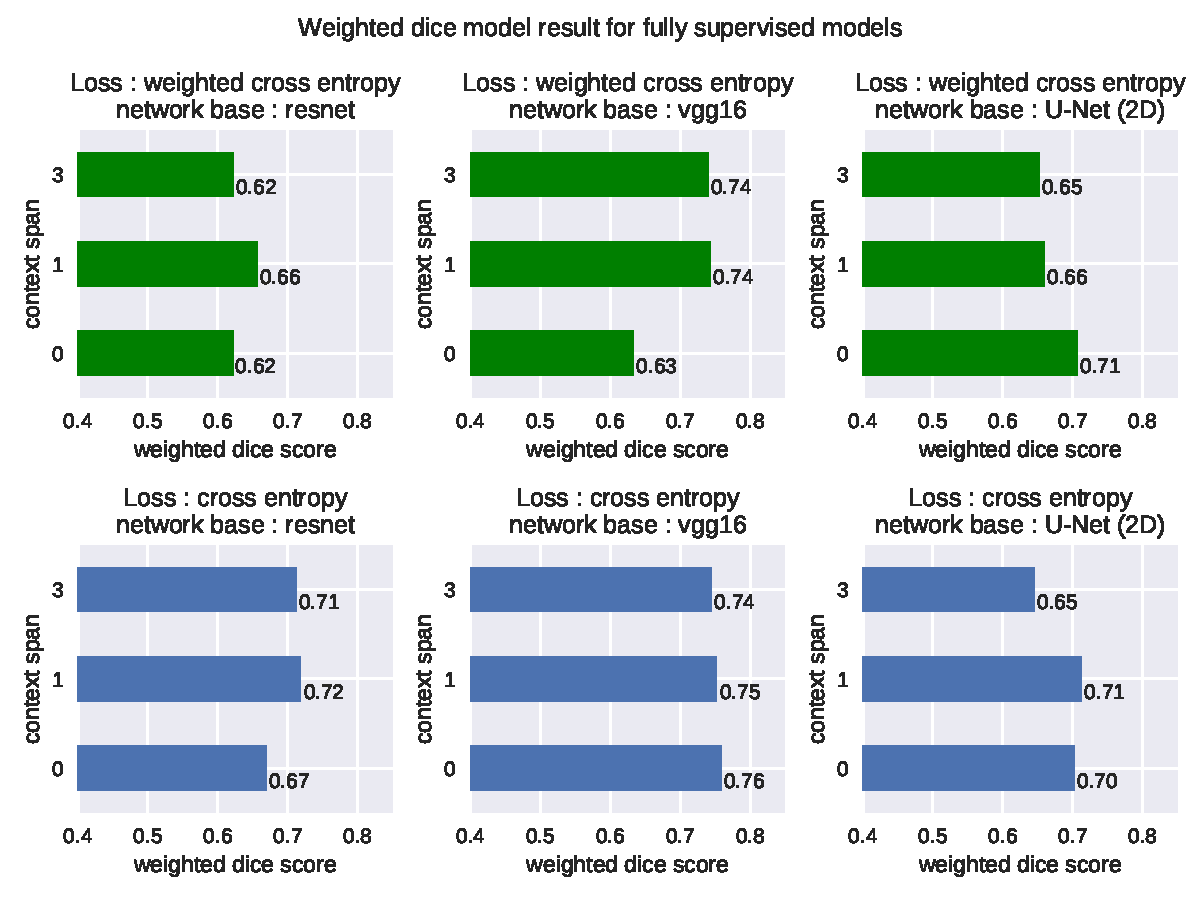
\includegraphics[width=.98\textwidth]{images/FullySupervised.pdf}
    \caption{Results of the fully supervised experiments.
    The indicated model performance metrics are calculated on the test set.
    The columns represent de weighted dice scores for models based on the same network architecture with different loss functions.
    \label{fig:referenceExperiments}}
\end{SCfigure}

\begin{SCfigure}[][htb]
    \centering
    \begin{minipage}{.98\textwidth}
        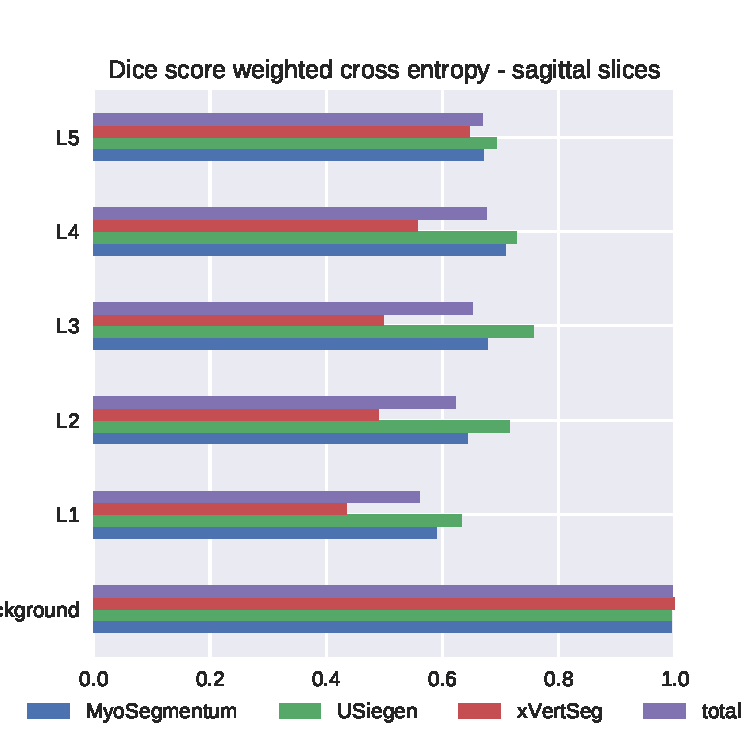
\includegraphics[width=.98\textwidth]{images/full_perClass_perSource_weighted.pdf}
    \end{minipage} 
    \begin{minipage}{0.98\textwidth}
        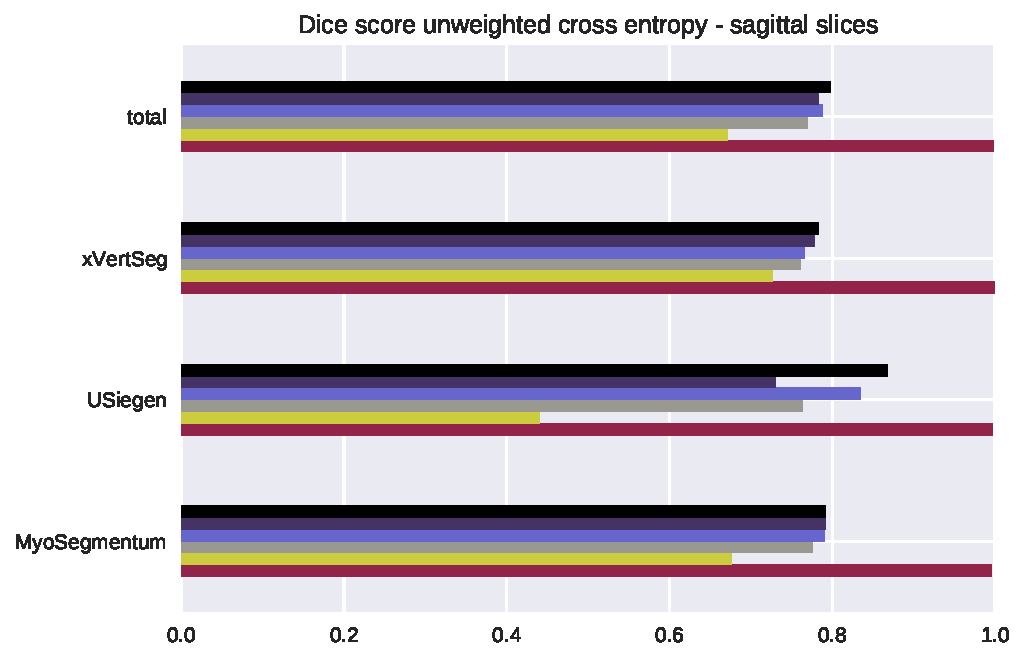
\includegraphics[width=.98\textwidth]{images/full_perClass_perSource_notweighted.pdf}
    \end{minipage}
    \caption{Detailed result for the fully supervised model trained without context slices and with a weighted cross entropy loss function.
    The model trained with the unweighted loss performs better than the result shown in figure \ref{fig:referenceWeighted} for the weighted cross entropy loss function.
    \label{fig:referenceWeighted} 
    }
\end{SCfigure}

\section{Conclusion}
\par{
    Based on the results shown in figure \ref{fig:referenceExperiments}, it was decided to perform the weakly supervised experiments with the model based on VGG16 FCN8 with one context slice.
    The reference performance metric to compare experiments with models trained on weakly supervised data is $\text{Dice}_{wi}=0,76$.
}




\chapter{Single dimension experiments \label{sec:singleDimension}}

\par{
    This chapter discusses the results of several experiments in the construction of single-dimensional models.
    The objective of these experiments is to investigate the influence different model hyperparameters have on the model performance.
    Based on this investigation, the hyperparameters for the single-dimensional models in the final step can be chosen.  
}

\section{Single dimension weakly supervised models}

\par{
    In this section, the results of experiments with different model hyperparameters are compared to each other.
    The point annotation sets are generated from the available full annotation masks for each slice.
    In this work, different datasets were used with different levels of provided annotation. 
    Annotation differences between different datasets are listed in table \ref{tab:datasetReferences} on page \pageref{tab:datasetReferences}.
}
\par{
    For three datasets\footnote{The three datasets for which complete annotation is available are the xVertSeg dataset, the UniSiegen dataset and the MyoSegmentum dataset. Of which the MyoSegmentum dataset is the largest by far.},
    full annotation masks are available, meaning that these scan volumes are labelled with volumes for each of the five lumbar vertebrae.
    For each voxel, the ground truth indicates whether it belongs to a lumbar vertebra and which vertebra.
    For one dataset (PLoS), only semantic segmentation is available. It means that the lumbar vertebrae are indicated as one class but not distinguished. 
    With each voxel in the PLoS dataset, ground truth is associated that indicates if it belongs to a lumbar vertebra. There is no label, however, to indicate which of the lumbar vertebrae this is.
}
\par{
    When a scan is sliced along the craniocaudal axis\footnote{
        The nomenclature of anatomical planes and axis is illustrated in figure \ref{fig:anatomicalPlains} on page \pageref{fig:anatomicalPlains}.
        The craniocaudal axis is the vertical axis when the patient is standing up.} 
    a human can distinguish all 5 lumbar vertebrae (after some practice).
    Therefore, one may hope the single-dimension models trained on sagittal or frontal slices will be able to do the same.
    Even though delineating a vertebra on a transverse slice is possible, identifying which vertebra is presented is challenging for a human.
    Supported by a brief test, it was confirmed that trying to estimate 5 vertebra classes from the transverse slices only provides very confusing results.
    The models trained on the transverse slices only intend to label the slice pixels as either background (0) or vertebra (1), 
    whereas the models trained on the sagittal and frontal slices intend to indicate which of 6 classes\footnote{0 for background, 1 for $L1$, 2 for $L2$, 3 for $L3$, 4 for $L4$ and 5 for $L2$} the pixel belongs to.
}
\par{
    The models trained to segment sagittal and frontal slices were trained on datasets xVertSeg, UniSiegen and MyoSegmenTUM.
    From the available full masks, point annotation labels were extracted.
    The models trained to segment transverse slices\footnote{This segmentation is, as stated not based on distinguishing separate lumbar vertebrae from each other.} 
    are trained on the same three datasets and additionally on the PLoS dataset.    
}
\par{
    The model performance results are compared based on the weighted dice score calculated on the test set.
    This metric is described in chapter \ref{sec:dice} on page \pageref{sec:dice}.
}


\subsection{Evaluation of the model Hyperparameters}

\par{
    To obtain the best model hyperparameters to train the single-dimension models, several tests were conducted to estimate the influence of model components and model hyperparameters\footnote{
        One could argue that the number of annotation points is not a \textit{model} hyperparameter. It is an essential parameter for the \textit{modelling} approach in general.
    } on the model performance.
}

\subsubsection{Weighted vs unweighted point loss performance}

\par{
    Equation \ref{eq:LP} on page \pageref{eq:LP} defines the point loss $\mathcal{L}_P$. 
    In this equation, the factor $w_{\mathcal{Y}_i(\vec{p})}$ indicates a weight that can be assigned to each of the output classes.
    Since data classes can be unbalanced, these weights can help to counter this imbalance.
    In this problem (based on the available datasets), there are about 500 times more background voxels than voxels belonging to a lumbar vertebra.
    By weighing with a factor proportional\footnote{The weighting vector is normalized.} to this ratio, this imbalance can be countered\footnote{
        When full data labels are available, the counts of the voxel types are available for the train set (one should not include the counts of the validation \& test set to avoid data leakage).
        In principle, this information is not necessarily available when only point level annotation is available. In this work, it is considered that (at least an approximation) of the ratios can be available as prior knowledge.
    }. In the unweighted case, $w_{\cdot} = 1$.
}
\par{
    In figure \ref{fig:weighted_vs_unweighted}, the difference between the weighted dice score \& the average dice score on the test set is compared for two models trained on the transverse slices.
    This result shows that the result of the non-weighted segmentation is better than the result of the model trained with weighted loss.
    Contrary to fully supervised models, in the weakly supervised case, the ratio between \textit{labelled} points is not as unbalanced as the ratio between the actual class pixels in the result.
    This explains the weighted point loss performance compared to the unweighted point loss performance.
    An approach that is not tested in this work is to weigh proportional to the inverse of the number of \textit{annotation} points per class instead of weighing proportional to the number of \textit{ground truth} pixels.
}


\begin{SCfigure}[][htb]
    \centering
    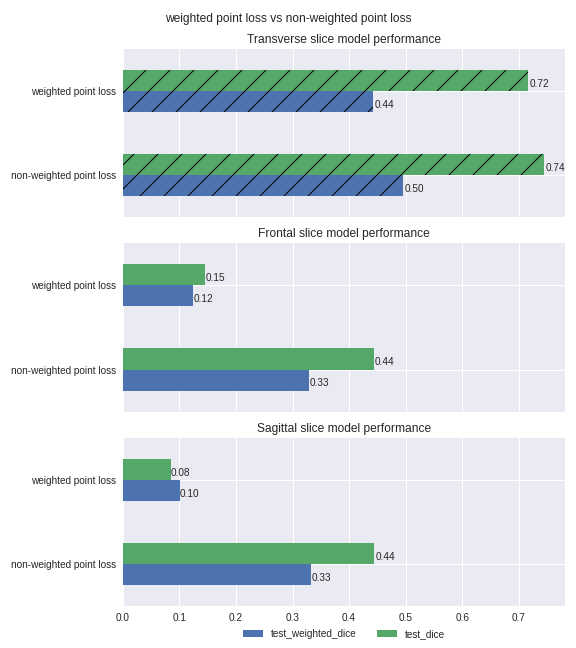
\includegraphics[width=.95\textwidth]{images/weightedvsnonweighted.png}
    \caption{Illustration of the difference in model performance between a weighted point loss function and the unweighted point loss function\label{fig:weighted_vs_unweighted}}
\end{SCfigure}

\subsubsection{Value of the added loss components}
\par{
    In this work, two-loss components were added to the consistency loss published in \cite{Laradji}.
    
    Where \cite{Laradji} is based only on the point loss $\mathcal{L}_P$ and the consistency loss $\mathcal{L}_C$, this work makes use of two extra loss components:
    the prior extend loss $\mathcal{L}_E$ and the separation loss $\mathcal{L}_S$. The four-loss components used in this work are described in more detail in \ref{sec:LossFunctions}.
    Figure \ref{fig:addedLossComponents} shows experimental results validating the positive influence these added loss terms have on the model performance.
}


\begin{SCfigure}[][htb]
    \centering
    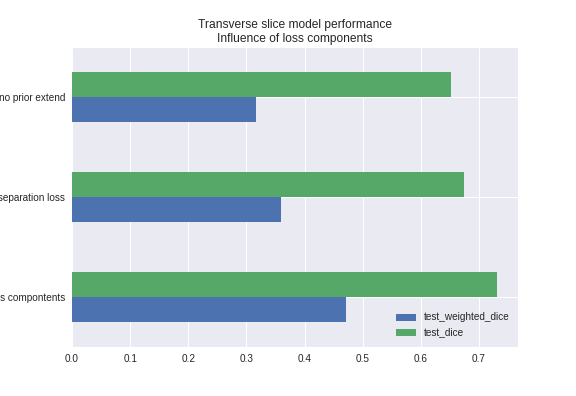
\includegraphics[width=.95\textwidth]{images/TransverseModel_Losscomponents.png}
    \caption{Evaluation of the added value of loss components. \label{fig:addedLossComponents}}
\end{SCfigure}

\subsection{Evolution of the model performance with increased labelling effort}
\par{
    The most basic modelling hyperparameter for a point annotation modelling campaign is the number of labelling points one asks the expert to provide.
    This section presents experimental results to estimate the influence of the number of annotation points on the resulting model performance.
    Intuitively, one would expect the model performance to increase with the number of annotation points provided.
    This hypothesis turns out to be false.
}
\begin{SCfigure}[][htb]
    \centering
    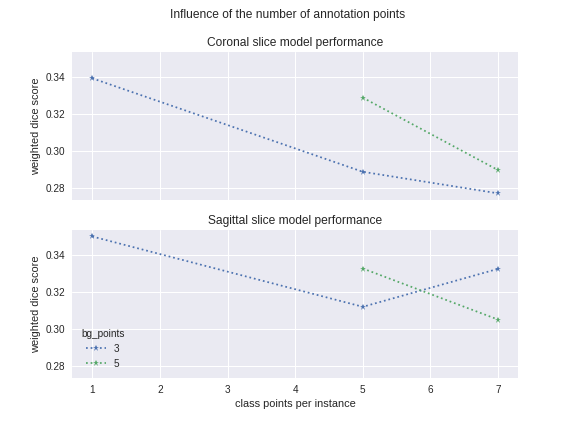
\includegraphics[width=.95\textwidth]{images/BlobPoints_influence.png}
    \caption{Evaluation of the added value of loss components. \label{fig:addedLossComponents}}
\end{SCfigure}
\par{
    Figure \ref{fig:addedLossComponents} shows the weighted dice score actually decreases with more annotation points.
    This is caused by the increased recall of the model. 
    The model becomes very eager to find class points, this causes a lot of background pixels to be wrongly classified as class points.
    The resulting decrease in precision causes the F1 score to decrease.
}
\todo[inline]{Werk verder uit met afbeelding en tabel}



\chapter{Single dimension model combination\label{sec:combination}}

All models are designed for $352 \times 352$ crops of the 2D slices.
The estimation of the slice is obtained by combining the model estimations on all crops taken from this slice.

\section{Volume combination procedure}

Combining the results of three different single dimension models is performed in two steps:
\begin{enumerate}
    \item The resulting classification volumes are first combined with a rule-based method
    \item After this rule-based combination, the resulting segmentation estimation is smoothened with a morphological filter.
\end{enumerate}

\subsection{Rule based result combination}
Three single dimension models are trained:
\begin{description}
    \item[Transverse slices] offer little context to indicate which of the lumbar vertebrae they contain. 
    It does not seem easy even for a human expert to indicate which vertebra is visible on the slice.
    The model trained on these slices is intended only for semantic segmentation.
    Each pixel is inferred only if it represents a vertebra, without distinction between the different lumbar vertebrae. 
    \item[Sagittal \& Coronal slices] do offer the necessary context to distinguish between $L_1$ to $L_5$. 
    The models trained on these slices do indicate the specific lumbar vertebra index. 
\end{description}

Based on the observation that all trained models accurately predict the background, these three models are combined in a straightforward way\footnote{
    The resulting estimations from a model for an input volume is again a three-dimensional volume ($\in \mathbb{N}^3$) with the same dimensions.
}.

\begin{algorithm}[H]
    \SetAlgoLined
    \KwData{
        Results $y_.$ of three models indicating an estimated class for all positions $\vec{p}$ in the volume.
        \begin{itemize} 
            \item Transverse model $y_t \in \mathbb{N}^3: \forall y_t(\vec{p}) \in \{ 0, 1 \}$
            \item Sagittal model $y_s \in \mathbb{N}^3: \forall y_t(\vec{p}) \in \{ 0, 1, 2, 3, 4, 5 \}$ 
            \item Coronal model $y_c \in \mathbb{N}^3: \forall y_t(\vec{p}) \in \{ 0, 1, 2, 3, 4, 5 \}$ 
        \end{itemize}
    }
    \KwResult{Combination of the three model results $y_f$.}
    \For{all $\vec{p}$}{
        \eIf{$y_t[\vec{p}] = 1 \wedge y_s[\vec{p}] = y_c[\vec{p}]$}{
            $y_f[\vec{p}] \leftarrow y_s[\vec{p}]$ \;
        }{
            $y_f[\vec{p}] \leftarrow 0$ \;
        }
    }
   \caption{Rule based combination of model results from three single dimension models}
\end{algorithm}

\todo[inline]{Image illustrating the combination}

\subsection{Morphological smoothing}
After the rule-based combination of estimations from different single dimension models, the result is smoothened with standard morphological filters.
These filters are combinations of the morphological \textit{erosion} and \textit{dilation} operators.
\todo[inline]{How deep should these morphological filters be discussed?}
\begin{itemize}
    \item Possible noise is suppressed by first opening and then closing the volumes.
    \item The estimated volumes are observed to overestimate the extent of the vertebrae. For this reason, an erosion step is performed to decrease the overall extent of the class masks.
\end{itemize}

The procedure mentioned above has two Hyperparameters: the number of iterations for the denoising filters and the number of iterations for the erosion filter.
Both hyperparameters are estimated by calculating the same evaluation metric, the weigh dice score on the validation set, as for the single-dimensional model evaluation. 


\begin{SCfigure}[][htb]
    \centering
    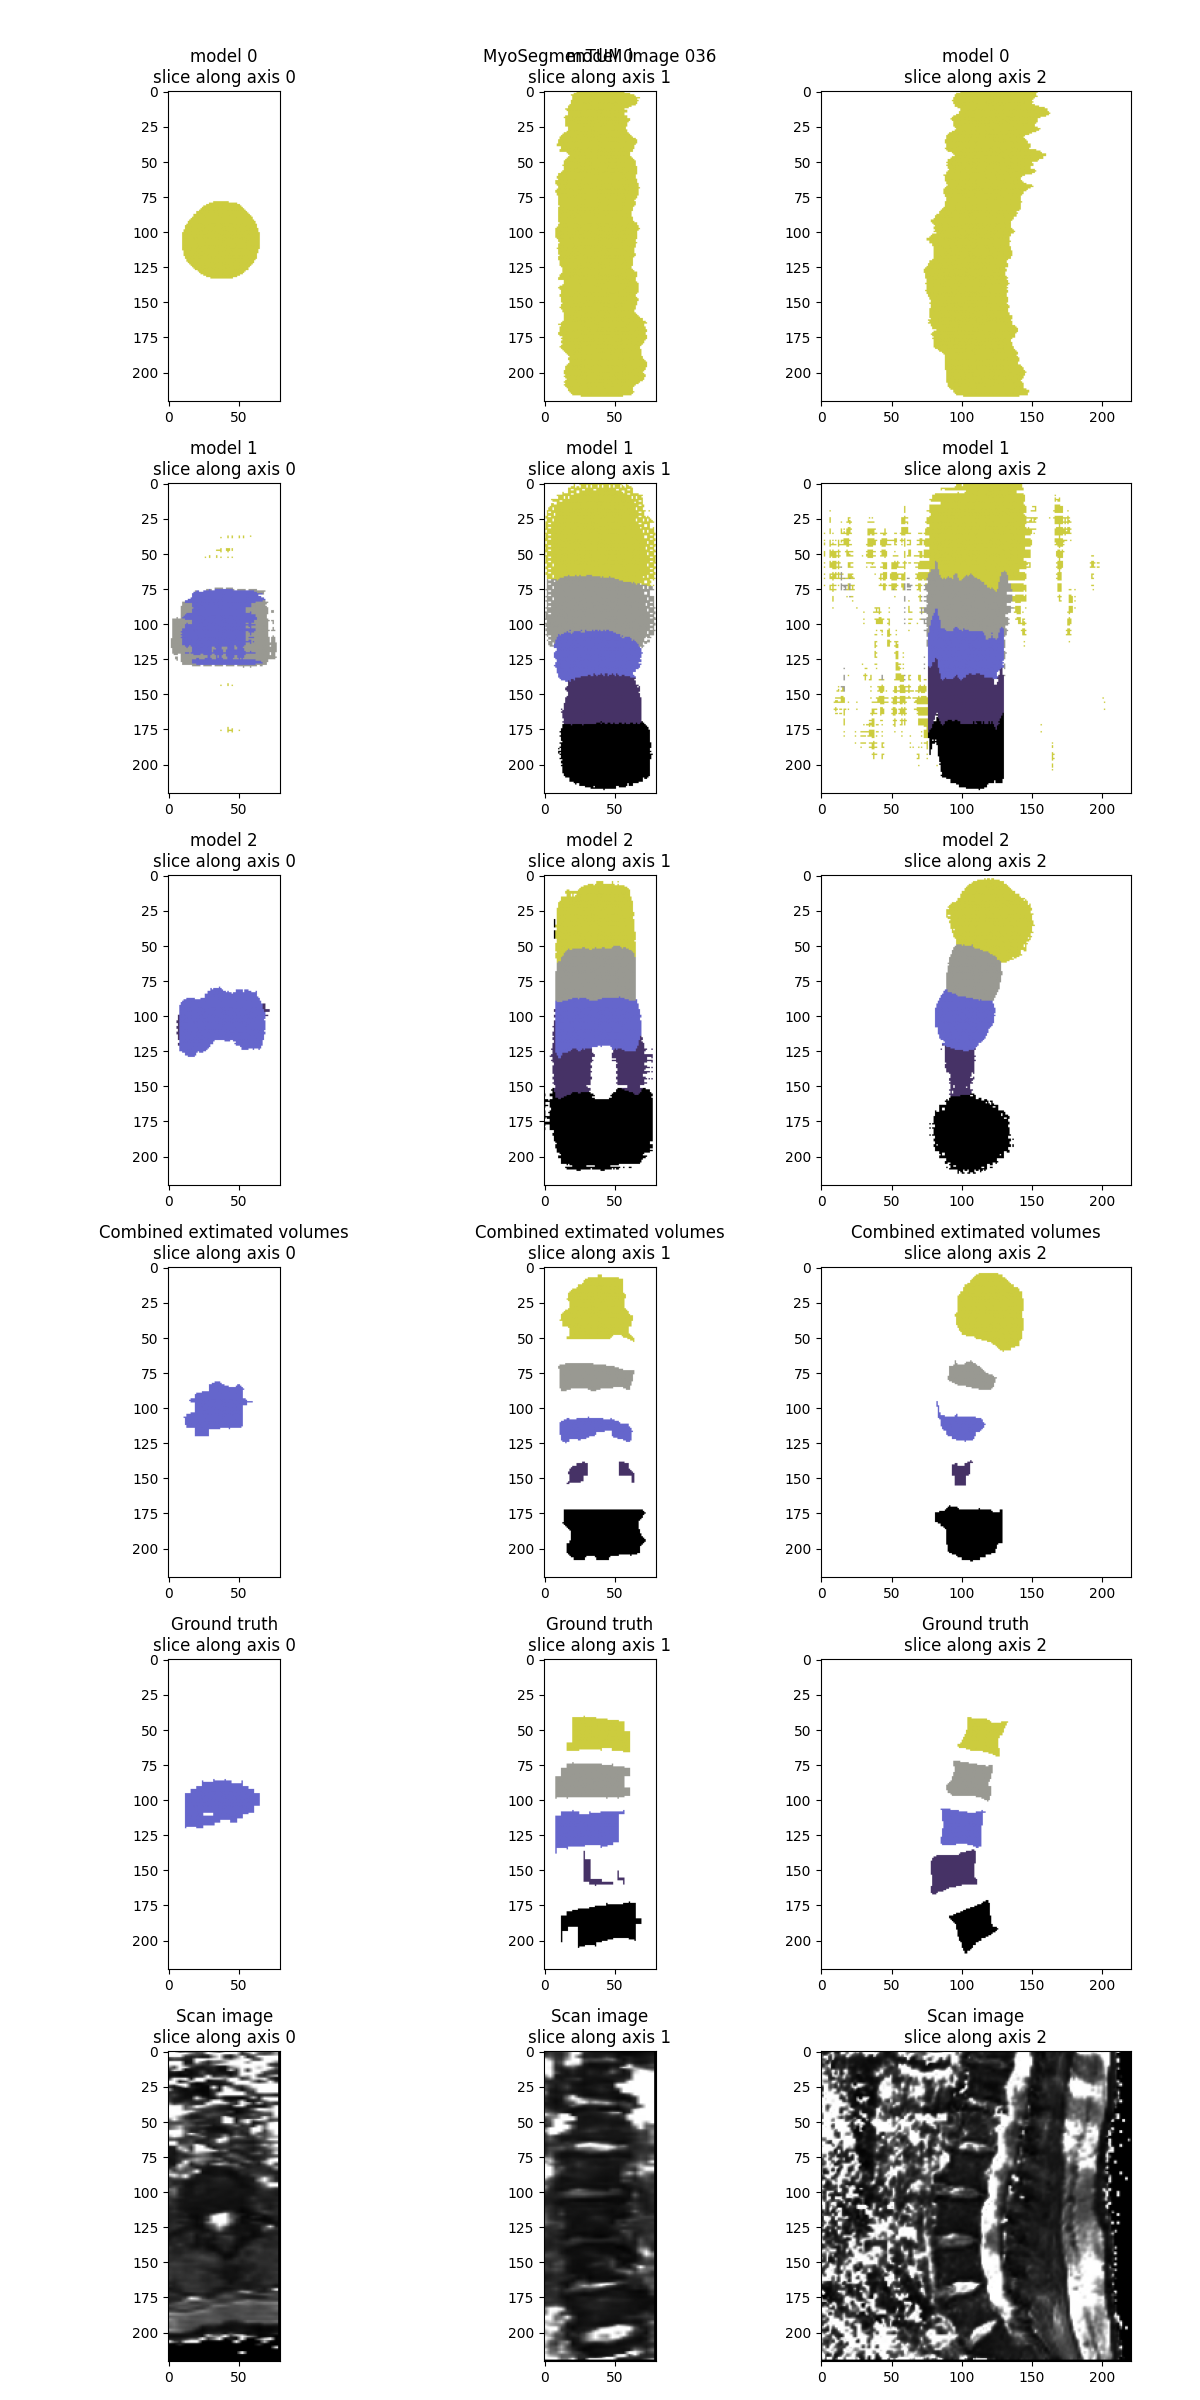
\includegraphics[width=.95\textwidth]{images/morphmask_denoise1_erode1_MyoSegmenTUM_036.png}
    \caption{
        Result of the combination of the three single dimension model results for volume MyoSegmenTUM nr 43.
        The colours indicate the vertebra classes. Only one semantic class is estimated in the first row, illustrating the model trained on transversal slices.
        On the first three rows, slices of the resulting segmentations from the single dimension models are shown. 
        It is clear these masks contain some artefacts and are not always in agreement with each other.
        On the fourth row, the result after mask combination and morphological smoothing is shown. 
        This corresponds more closely to the ground truth mask, shown on the fifth row.
        This final mask, shown on the fourth row, will be used as a pseudo mask to approximate the unknown ground truth mask.
        In the last row, the corresponding images are shown.
    }
\end{SCfigure}

\section{Pseudo mask performance}

\chapter{Pseudo mask training}

Time to evaluate
performance